% Sandia National Laboratories is a multimission laboratory managed and
% operated by National Technology & Engineering Solutions of Sandia, LLC, a
% wholly owned subsidiary of Honeywell International Inc., for the U.S.
% Department of Energy’s National Nuclear Security Administration under
% contract DE-NA0003525.

% Copyright 2002-2019 National Technology & Engineering Solutions of Sandia,
% LLC (NTESS).


%%
%% Mutal Inductor Table
%%
\small
\begin{longtable}[Hh]{>{\setlength{\hsize}{.2\hsize}}YY} \hline

\underline{\bf General Form} &
\verb|K<name> L<inductor name> [L<inductor name>*] <coupling value>|
\verb|+ [model name] | \\ \hline

\underline{\bf Examples} &
\begin{alltt}
KTUNED L3OUT  L4IN .8
KTRNSFRM LPRIMARY LSECNDRY 1
KXFRM L1 L2  L3  L4 .98 KPOT\_3C8
\end{alltt} \\ \hline

\underline{\bf Symbol} &
{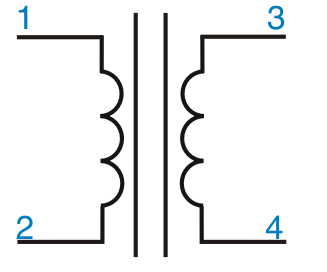
\includegraphics{transformerSymbol}}
\\ \hline

\underline{\bf Model Form} &
\verb|.MODEL <model name> CORE [model parameters]| \\ \hline

\underline{\bf Parameters} \underline{\bf and Options} &
\texttt{L<inductor name> [L<inductor name>*]}
\begin{quote}
  Identifies the inductors to be coupled. The inductors are coupled and in
  the dot notation the dot is placed on the first node of each inductor. The
  polarity is determined by the order of the nodes in the L devices and not by
  the order of the inductors in the K statement.
\end{quote}
\texttt{<coupling value>}
\begin{quote}
  The coefficient of mutual coupling, which must be between $-1.0$
  and $1.0$.

  This coefficient is defined by the equation
  \begin{quote}
    \texttt{<coupling value>} = $\frac{M_{ij}}{\sqrt{L_iL_j}}$
  \end {quote}

  where
  \begin{quote}
    $L_i$ is the inductance of the $i$th named inductor in the K-line
  \end {quote}
  \begin{quote}
    $M_{ij}$ is the mutual inductance between $L_i$ and $L_j$
  \end {quote}
  For transformers of normal geometry, use $1.0$ as the value. Values less
  than $1.0$ occur in air core transformers when the coils do not completely
  overlap.
\end{quote}
\texttt{<model name>}
\begin{quote}
  If \texttt{<model name>} is present, four things change:
  \begin{itemize}
    \item The mutual coupling inductor becomes a nonlinear, magnetic core device.
    \item The inductors become windings, so the number specifying inductance now
          specifies the number of turns.
    \item The list of coupled inductors could be just one inductor.
    \item A model statement is required to specify the model parameters.
  \end{itemize}
\end{quote}
\\ \hline

\end{longtable}

% Eric Keiter.  1/19/04:
% As this table does not have a caption, it should not have a number
% assigned to it.  This line is needed to fix latex so that the tables in
% chapter 2, which actually have their numbers printed in table captions, 
% and the list of tables,  do not start at 2.9, but start at 2.1.
\addtocounter{table}{-1}

